\documentclass[
11pt, % The default document font size, options: 10pt, 11pt, 12pt
codirector, % Uncomment to add a codirector to the title page
]{charter} 

% El títulos de la memoria, se usa en la carátula y se puede usar el cualquier lugar del documento con el comando \ttitle
\titulo{Título del proyecto} 

% Nombre del posgrado, se usa en la carátula y se puede usar el cualquier lugar del documento con el comando \degreename
\posgrado{Carrera de Especialización en Sistemas Embebidos} 
%\posgrado{Carrera de Especialización en Internet de las Cosas} 
%\posgrado{Carrera de Especialización en Intelegencia Artificial}
%\posgrado{Maestría en Sistemas Embebidos} 
%\posgrado{Maestría en Internet de las cosas}

% Tu nombre, se puede usar el cualquier lugar del documento con el comando \authorname
\autor{SISE-RS versión B} 

% El nombre del director y co-director, se puede usar el cualquier lugar del documento con el comando \supname y \cosupname y \pertesupname y \pertecosupname
\director{Nombre del Director}
\pertenenciaDirector{pertenencia} 
% FIXME:NO IMPLEMENTADO EL CODIRECTOR ni su pertenencia
\codirector{John Doe} % para que aparezca en la portada se debe descomentar la opción codirector en el documentclass
\pertenenciaCoDirector{FIUBA}

% Nombre del cliente, quien va a aprobar los resultados del proyecto, se puede usar con el comando \clientename y \empclientename
\cliente{Nombre del cliente}
\empresaCliente{Empresa del cliente}

% Nombre y pertenencia de los jurados, se pueden usar el cualquier lugar del documento con el comando \jurunoname, \jurdosname y \jurtresname y \perteunoname, \pertedosname y \pertetresname.
\juradoUno{Nombre y Apellido (1)}
\pertenenciaJurUno{pertenencia (1)} 
\juradoDos{Nombre y Apellido (2)}
\pertenenciaJurDos{pertenencia (2)}
\juradoTres{Nombre y Apellido (3)}
\pertenenciaJurTres{pertenencia (3)}
 
\fechaINICIO{30 de abril de 2021}		%Fecha de inicio de la cursada de GdP \fechaInicioName
\fechaFINALPlan{18 de junio de 2021} 	%Fecha de final de cursada de GdP
\fechaFINALTrabajo{15 de mayo de 2022}	%Fecha de defensa pública del trabajo final

\def\codigo{SISE-RS}
\newcommand{\req}[1]{\textbf{[\codigo-#1]:}}

\begin{document}

\maketitle
\thispagestyle{empty}
\pagebreak


\thispagestyle{empty}
{\setlength{\parskip}{0pt}
\tableofcontents{}
}
\pagebreak


\section*{Registros de cambios}
\label{sec:registro}

\begin{table}[ht]
\label{tab:registro}
\centering
\begin{tabularx}{\linewidth}{@{}|c|X|c|@{}}
\hline
\rowcolor[HTML]{C0C0C0} 
Revisión & \multicolumn{1}{c|}{\cellcolor[HTML]{C0C0C0}Detalles de los cambios realizados} & Fecha      \\ \hline
A & Creación del documento & 27/06/2021 \\ \hline
B & Se agrega encabezado en la plantilla del documento. \newline
	Modificación de la tabla de registro de cambios. \newline
	Nuevo formato de enumeración de requisitos.\newline
	Se amplia la sección \ref{sub:perspectiva}. & 03/07/2021 \\ \hline
\end{tabularx}
\end{table}

\pagebreak

\section{1. Introducción}
\label{sec:introduccion}

\subsection{Propósito}
\label{sub:proposito}

Este documento representa una especificación de requerimientos de software para un sistema de inyección de \emph{soft-errors} y un \emph{firmware} de \emph{self-testing}.
Está dirigido a las personas que se ocupen de las siguientes tareas:
\begin{itemize}
	\item análisis
	\item diseño
	\item implementación
	\item pruebas
\end{itemize}

\subsection{Ámbito del sistema}
\label{sub:ambito}

El nombre del sistema será SISE y permitirá inyectar errores en todos los registros accesibles del microcontrolador \emph{SAMV71}.
Su función será evaluar las técnicas de mitigación de \emph{soft-errors} en funciones a ser utilizadas en la misión \emph{Sabiamar}.
Adicionalmente, se proveerá un \emph{firmware} de \emph{self-testing} para determinar los presupuestos de \emph{hardware}.

El beneficio que se espera obtener es utilizar componentes que no fueron sometidos a un proceso de calificación (alternativos).
Además, se espera simular los 5 años de misión en un tiempo acelerado.

\subsection{Definiciones, acrónimos y abreviaturas}
\label{sub:definiciones}

\begin{enumerate}
	\item Definiciones:
		\begin{itemize}
			\item Sabiamar: constelación de dos satélites argentino-brasileños para la información del mar.
			\item soft-errors: modificación no destructiva del valor de un registro o memoria.
		\end{itemize}
	\item Acrónimos:
		\begin{itemize}
			\item CSV: comma separated value.
			\item IEEE: Institute of Electrical and Electronics Engineers.
			\item JTAG: Join Test Action Group.
			\item RAM: random access memory.
			\item TCP: transfer control protocol.
		\end{itemize}
	\item Abreviaturas:
		\begin{itemize}
			\item Std: estándar.
		\end{itemize}
\end{enumerate}

\subsection{Referencias}
\label{sub:referencias}
INVAP - Propuesta de tesis: sistema de inyección de soft-errors.

\subsection{Visión general del documento}
\label{sub:vision}

Este documento se realizó según lo especificado en el estándar IEEE Std. 830-1998.

\newpage
\section{2. Descripción general}
\label{seb:descripcion}

\subsection{Perspectiva del producto}
\label{sub:perspectiva}

El software aquí especificado es independiente de otros sistemas y no tiene relación con otros productos.

El principio de inyección de \emph{soft-erros} se basará en conectarse al microcontrolador a través de su interfaz de \emph{debug}; se procederá a suspender la ejecución del \emph{firmware} y luego se realizarán las modificaciones necesarias.

En la figura \ref{fig:esqInyeccion} se puede observar un esquema general del proceso de inyección de \emph{soft-errors}.

\begin{figure}[h]
	\centering
	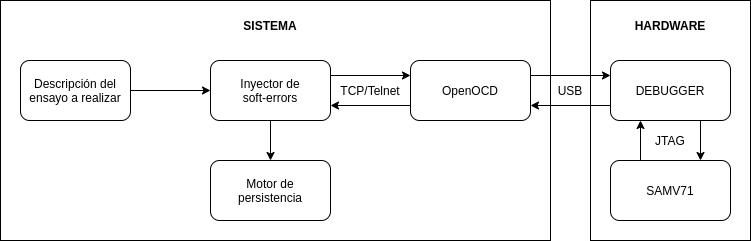
\includegraphics[width=\textwidth]{./Figuras/inyeccion.png}
	\caption{Esquema general de inyección de \emph{soft-errors}.}
	\label{fig:esqInyeccion}
\end{figure}

El inyector de \emph{soft-errors} deberá modificar obtener la información de los registros del microcontrolador SAMV71 antes de realizar una modificación.
Finalmente, debe persistir la operación realizada junto a los datos previos a la inyección.

Adicionalmente, se entregará un \emph{firmware} de \emph{self-testing} que generará reportes sobre el funcionamiento de los periféricos del microcontrolador \emph{SAMV71}.
En la figura \ref{fig:esqSelfTesting} se puede ver un esquema general del proceso de \emph{self-testing}.

\begin{figure}[h]
	\centering
	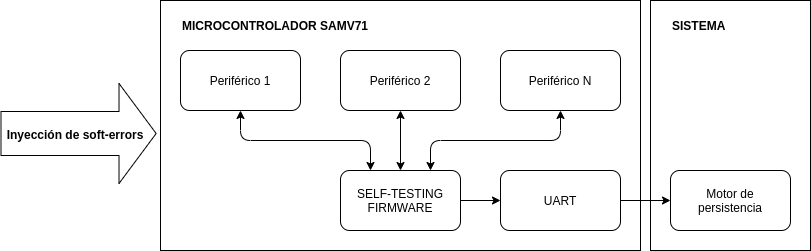
\includegraphics[width=\textwidth]{./Figuras/selfTesting.png}
	\caption{Esquema general del proceso de \emph{self-testing}.}
	\label{fig:esqSelfTesting}
\end{figure}

\subsection{Funciones del producto}
\label{sub:funcionesProducto}

El software aquí especificado brindará las siguientes funcionalidades:

\begin{itemize}
	\item Inyección de errores en todos los registros accesibles del microcontrolador SAMV71.
	\item Monitoreo del estado de funcionamiento del microcontrolador SAMV71.
	\item Persistencia de los soft-errors inyectados.
	\item Persistencia de los informes de estado de funcionamiento.
	\item Permitir escribir ensayos de evaluación.
	\item Presentación de resultados en histogramas que permitan un análisis estadístico.
\end{itemize}

\subsection{Características de los usuarios}
\label{sub:usuarios}

Los usuarios finales de este producto son ingenieros de desarrollo del INVAP.

\subsection{Restricciones}
\label{sub:restricciones}

Las restricciones del desarrollo del sistema son las siguientes:

\begin{itemize}
	\item Utilización de repositorio con control de versiones \emph{Gitlab}.
	\item Documentación del código con \emph{Doxygen}.
	\item Utilización exclusiva del lenguaje de programación \emph{Python 3}.
\end{itemize}

\subsection{Suposiciones y dependencias}
\label{sub:suposiciones}

La suposición principal es que se tendrá acceso irrestricto al microcontrolador \emph{SAMV71} antes del día 01/11/2021.

\subsection{Requisitos futuros}
\label{sub:futuro}

N/A

\newpage
\section{3. Requisitos específicos}
\label{sec:requisitos}


\subsection{Interfaces externas}
\label{sub:interfaces}

\begin{itemize}
	\item \req{001} se comunicará de forma bidireccional con \emph{OpenOCD} a través de \emph{TCP} o \emph{Telnet}.
	\item \req{002} se deberá recibir y capturar la información proveniente por puerto \emph{Serial} del microcontrolador \emph{SAMV71}.
\end{itemize}

\subsection{Funciones}
\label{sub:funciones}

\begin{enumerate}
	\item Inyección de \emph{soft-errors}:
	\begin{itemize}
		\item \req{003} sobrescribirá los valores en memoria \emph{RAM}.
		\item \req{004} invertirá el valor de un bit en la memoria \emph{RAM}.
		\item \req{005} sobrescribirá valores en los registros internos.
		\item \req{006} invertirá el valor de un bit dentro de un registro interno.
		\item \req{007} reportará el estado del microcontrolador antes de realizar una inyección de \emph{soft-errors}.
		\item \req{008} interpretará una descripción de ensayo escrita en \emph{Python 3} y ejecutará las inyecciones según le indique.
		\item \req{009} aceptará descripciones de ensayo que impongan una tasa de error para cada registro interno.
		\item \req{010} procesará descripciones de ensayo que impongan una tasa de error para una posición o rango de memoria \emph{RAM}.
		\item \req{011} las descripciones de ensayo podrán especificar probabilidades de error con una resolución de 1 bit.
	\end{itemize}
	\item \emph{Firmware} de \emph{self-testing}:
	\begin{itemize}
		\item \req{012} detectará el funcionamiento anormal de los periféricos del microcontrolador \emph{SAMV71}.
		\item \req{013} reportará periódicamente el estado de los periféricos utilizando el protocolo \emph{Serial}.
		\item \req{014} los reportes tendrán un formato \emph{CSV} y un tamaño menor a 5 kB.
	\end{itemize}
	\item Almacenamiento de reportes:
	\begin{itemize}
		\item \req{015} se incluirá un \emph{timestamp} de recepción del reporte.
		\item \req{016} se generarán histogramas para su análisis estadístico.
	\end{itemize}
\end{enumerate}

\subsection{Requisitos de rendimiento}
\label{sub:rendimiento}

\req{017} el inyector de soft-errors deberá realizar la inserción solicitada en un tiempo menor a 10 ms.

\subsection{Restricciones de diseño}
\label{sub:restriccionesDiseño}

\req{018} se utilizará el microcontrolador \emph{SAMV71} como dispositivo principal.

\subsection{Atributos del sistema}
\label{sub:atributos}

\begin{enumerate}
	\item Mantenibilidad:
	\begin{itemize}
		\item \req{019} el software deberá permitir su modificación para trabajar con otras arquitecturas.
	\end{itemize}
\end{enumerate}

\subsection{Otros requisitos}
\label{sub:otros}

N/A.

\section{4. Apéndices}
\label{sec:apendices}

%\subsection{Formatos de entrada/salida}¸

%\subsection{Resultados de análisis de costes}

\subsection{Restricciones acerca del lenguaje de programación}

El lenguaje de programación será \emph{Python 3} y el código deberá ser documentado según las recomendaciones del manual de usuario de \emph{Doxygen}.

\subsection{Casos de uso}

\begin{table}[h!]
	\label{tab:uso1}
	\caption{Caso de uso número 1}
	\begin{tabularx}{\textwidth}{|ll|X|}
		\hline
		\rowcolor[HTML]{C0C0C0} 
		\multicolumn{2}{|c|}{\cellcolor[HTML]{C0C0C0}\textbf{Título}} & \multicolumn{1}{c|}{\cellcolor[HTML]{C0C0C0}\textbf{Descripción}} \\ \hline
		\multicolumn{2}{|l|}{1. Nombre}                               & Simular misión Sabiamar                                           \\ \hline
		& 1.1 Breve descripción                   & Se simulan los 5 años de \emph{soft-errors} en un lapso de 24 horas                   \\ \hline
		& 1.2 Actor principal                     & Usuario del sistema                                                                   \\ \hline
		& 1.3 Disparadores                        & Comando de ejecución                                                                  \\ \hline
		\multicolumn{2}{|l|}{2. Flujo de eventos} &                                                                                       \\ \hline
		& 2.1 Flujo básico                        & \begin{tabular}[c]{@{}l@{}}
			                                                       1. El software interpreta la descripción del ensayo                    \\ 
			                                                       2. El software determina la tasa de falla del ensayo                   \\ 
			                                                       3. El software determina la probabilidad de falla de cada registro     \\
			                                                       4. El software determina la probabilidad de falla en memoria           \\
			                                                       5. El software realiza inyecciones según los parámetros calculados     \\
			                                                       6. El software persiste todas las inyecciones realizadas               \\
			                                                       7. El software entrega un informe final                                \\
			                                                       8. El software retorna un código de tarea finalizada
		                                            \end{tabular} \\ \hline
		& 2.2 Fuljo alternativo                   & \begin{tabular}[c]{@{}l@{}}
			                                                       1. El software detecta una anormalidad en el ensayo                    \\ 
			                                                       2. El software aborta el ensayo                                        \\ 
			                                                       3. El software genera un informe de fallo                              \\
			                                                       4. El software retorna un código de error
		                                            \end{tabular} \\ \hline
		\multicolumn{2}{|l|}{3. Pre-condiciones}  & \begin{tabular}[c]{@{}l@{}}
                                                                   1. \emph{OpenOCD} corriendo                                            \\ 
                                                                   2. \emph{OpenOCD} conectado al microcontrolador                        \\ 
                                                                   3. \emph{OpenOCD} con puerto disponible
													\end{tabular}\\ \hline
		\multicolumn{2}{|l|}{4. Pos-condiciones}  & \emph{OpenOCD} con puerto liberado                                                    \\ \hline
	\end{tabularx}
\end{table}

\begin{table}[h!]
	\label{tab:uso2}
	\caption{Caso de uso número 2}
	\begin{tabularx}{\textwidth}{|ll|X|}
		\hline
		\rowcolor[HTML]{C0C0C0} 
		\multicolumn{2}{|c|}{\cellcolor[HTML]{C0C0C0}\textbf{Título}} & \multicolumn{1}{c|}{\cellcolor[HTML]{C0C0C0}\textbf{Descripción}}  \\ \hline
		\multicolumn{2}{|l|}{1. Nombre}                               & Validación de hardware                                             \\ \hline
		& 1.1 Breve descripción                   & Se prueba la capacidad de los periféricos del microcontrolador para reponerse de fallas\\ \hline
		& 1.2 Actor principal                     & Banco de pruebas INVAP                                                                 \\ \hline
		& 1.3 Disparadores                        & Anormalidad en periférico                                                              \\ \hline
		\multicolumn{2}{|l|}{2. Flujo de eventos} &                                                                                        \\ \hline
		& 2.1 Flujo básico                        & \begin{tabular}[c]{@{}l@{}}
			                                                       1. El firmware detecta una anormalidad en un periférico                 \\ 
			                                                       2. El firmware genera un informe en formato \emph{CSV}                  \\ 
			                                                       3. El firmware envía un reporte por \emph{UART}                         \\
		                                            \end{tabular} \\ \hline
		& 2.2 Fuljo alternativo                   & \begin{tabular}[c]{@{}l@{}}
			                                                       1. El microcontrolador se reinicia                                      \\ 
			                                                       2. El firmware genera un informe en formato \emph{CSV}                  \\ 
			                                                       3. El firmware envía un reporte por \emph{UART}
		                                            \end{tabular}                                                                          \\ \hline
		\multicolumn{2}{|l|}{3. Pre-condiciones}  &                                                                                        \\ \hline
		\multicolumn{2}{|l|}{4. Pos-condiciones}  &                                                                                        \\ \hline
	\end{tabularx}
\end{table}



\end{document}
